\begin{figure}[h!]
  \centering    
    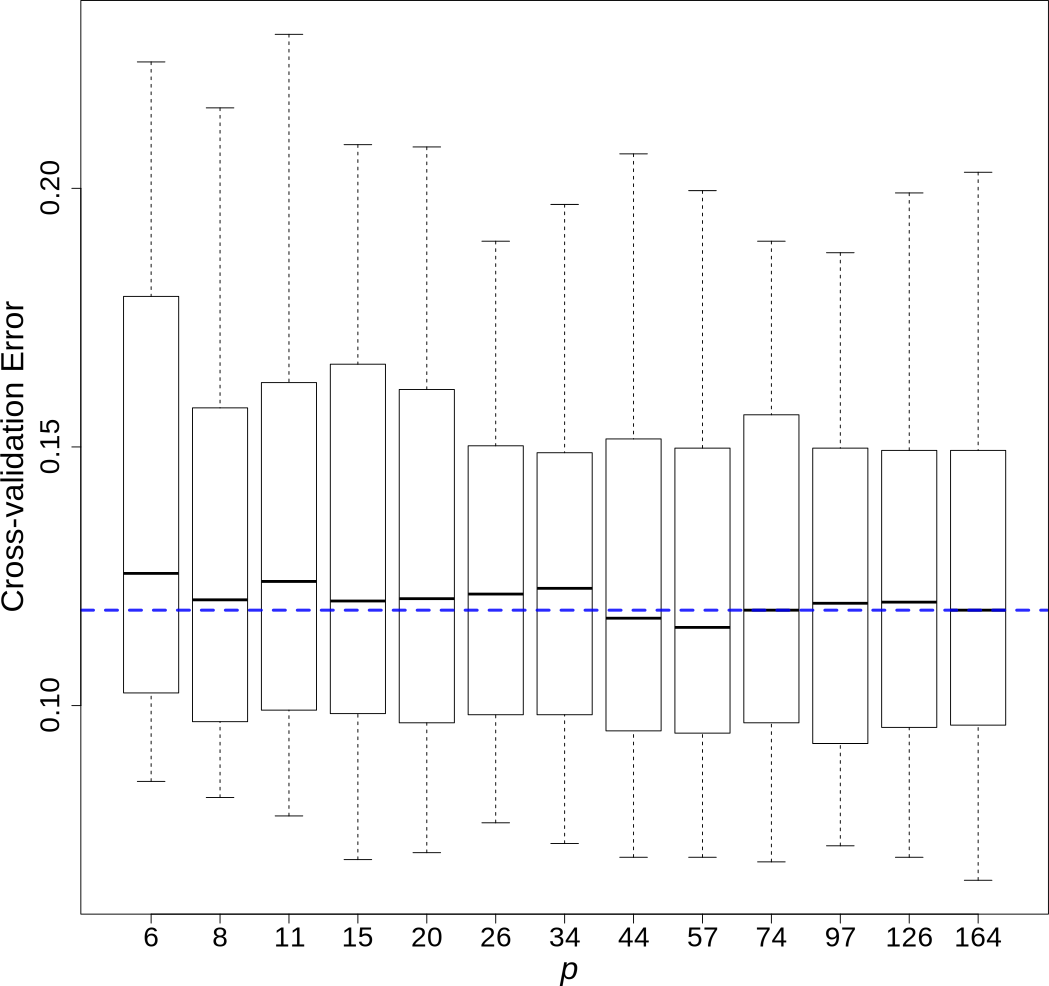
\includegraphics[width=0.5\textwidth]{figures/variable_elimination.pdf}
  \caption{\ctit{Recursive variable elimination.}
  Random forests were recursively fitted and, at each step, only the most important $p/1.5$ variables were kept.
  Stratified cross-validation (see Material and Methods) was computed at each iteration. This procedure was replicated five time.
  The dashed blue line ($y=0.12$) indicates the median cross-validation error when all variable are used.
  \label{fig:variable_elimination}
  }
\end{figure}
